\documentclass{standalone}
\usepackage{ctex}
\usepackage{tikz}
\usetikzlibrary{patterns}
\usetikzlibrary{decorations.pathmorphing}
\begin{document}

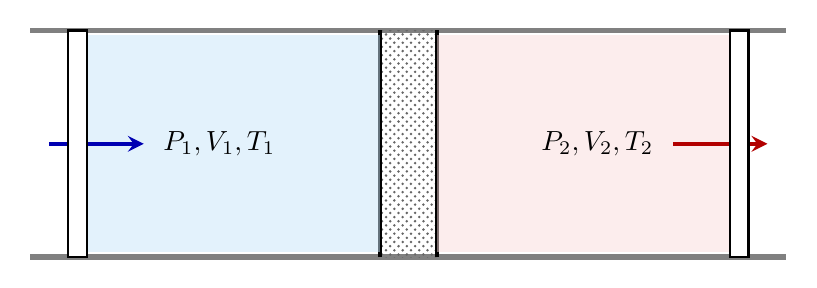
\begin{tikzpicture}[scale=1.2, thick]
    % 定义颜色
    \definecolor{gasblue}{RGB}{200, 230, 250}
    \definecolor{gasred}{RGB}{250, 220, 220}

    % 绝热管道外部结构
    \draw[line width=2pt, gray] (-4, 1.2) -- (4, 1.2);
    \draw[line width=2pt, gray] (-4, -1.2) -- (4, -1.2);
    
    % 填充绝热阴影 (Insulation)
    % \foreach \y in {1.2, -1.2} {
    %     \draw[decorate, decoration={zigzag, amplitude=0.5pt, segment length=5pt}] (-4, \y) -- (4, \y);
    %     \fill[pattern=north east lines, pattern color=gray!40] (-4, \y) rectangle (4, \y+0.3);
    %     \fill[pattern=north east lines, pattern color=gray!40] (-4, \y) rectangle (4, \y-0.3);
    % }

    % 多孔介质 (Porous Plug)
    \fill[pattern=crosshatch dots, pattern color=black!60] (-0.3, -1.2) rectangle (0.3, 1.2);
    \draw[line width=1.5pt] (-0.3, -1.2) -- (-0.3, 1.2);
    \draw[line width=1.5pt] (0.3, -1.2) -- (0.3, 1.2);
    % \node at (0, 1.6) {\small \textbf{多孔介质 (Porous Plug)}};

    % 左侧区域 (State 1)
    \fill[gasblue, opacity=0.5] (-3.5, -1.15) rectangle (-0.3, 1.15);
    \node[align=center] at (-2, 0) {$P_1, V_1, T_1$};
    \draw[->, >=stealth, blue!70!black, line width=1.5pt] (-3.8, 0) -- (-2.8, 0);

    % 右侧区域 (State 2)
    \fill[gasred, opacity=0.5] (0.3, -1.15) rectangle (3.5, 1.15);
    \node[align=center] at (2, 0) {$P_2, V_2, T_2$};
    \draw[->, >=stealth, red!70!black, line width=1.5pt] (2.8, 0) -- (3.8, 0);

    % 活塞示意 (Pistons)
    \draw[fill=white] (-3.6, -1.2) rectangle (-3.4, 1.2);
    \draw[fill=white] (3.4, -1.2) rectangle (3.6, 1.2);
    
    % % 绝热标注
    % \node at (0, -1.8) {\small \textbf{绝热壁 ($Q=0, H=$ const.)}};
    
\end{tikzpicture}

\end{document}